\chapter{Aplikace metod}

V této kapitole se budeme zabývat aplikováním a porovnáváním metod, kterým jsme se věnovali v kapitole \ref{chap:reseniOptUloh}.
Synteticky vygenerujeme data, která budou reprezentovat prostředky pohotovostní služby a sady incidentů. 
V rámci této práce budeme modelovat Pražskou záchranou službu pro rok 2017, podle veřejně dostupných dat
poskytnutých přímo ze zdravotnické záchranné služby hlavního města Prahy.
\footnote{https://www.zzshmp.cz/wp-content/uploads/2017/12/Statistiky-160let-ZZSHMP.pdf}.
Chování nalezených optimálních plánů budeme následně zkoumat na různých sadách incidentů.

\section{Generování dat}

První vygenerujeme data reprezentující výjezdové stanice a nemocnice a tím namodelujeme pohotovostní službu.
Ty můžeme v podstatě vygenerovat libovolně, ale v rámci praktičtějšího využití
si v této prácí vybereme jako pohotovostní službu Pražskou záchrannou službu.
Pražská záchranná služba disponuje 20 výjezdovými stanicemi a 140 vozidly.
Údaje o počtu záchranných týmu se zdají, že nejsou veřejně dostupné. Jedinou dostupnou informací je celkový počet zaměstanců, který činí přes 500 lidí.
Tam ale spadají i nezáchranáři.
V Praze se nachází 12 nemocnic.

Nyní namodelujeme incidenty. Podle statistik zveřejněných Pražskou záchrannou službou se v roce 2017 v Praze denně uskutečnilo na 330 výjezdů.
Nejrušnější část všedního dne je mezi 9 a 12 hodinou, kdy se odehrává až dvojnásobně incidentů než je průměr.
Incidenty se odehrávají mnohem častěji v centru a ve středu Prahy, než na jeho okolí. 

Podle těchto informací namodelujeme sadu incidentů.
První si území Prahy reprezentujeme jako polygon a pomocí normálního rozdělení vygenerujeme souřadnice v něm obsažené.
Normálnímu rozdělení nastavíme střední hodnotu na střed polygonu a směrodatnou odchylku nastavíme tak, aby se incidenty na okrajích Prahy odehrávali méně než v centru. 
Kde a v kolik hodin se incidenty odehrávají přesně záchranná služba Prahy vypadá, že nezveřejňuje, pravděpodobně proto, že by se mohlo jednat o zneužitelné nebo citlivé údaje.
Rozloha Prahy činí 496 kilometrů čtverečních a je poměrně symetrického tvaru. Pro naše účely tak bude stačit nastavit směrodatnou odchylku na 10 kilometrů.
V jakých časech se incidenty odehrávají je vygenerováno uniformě náhodně tak, aby se skutečně odehrávali incidenty častěji mezi 9 a 12 hodinou.

\begin{figure}[H]
  \caption{Záchranná pohotovostní služba a nemocnice spolu s incidenty na mapě Prahy.}
  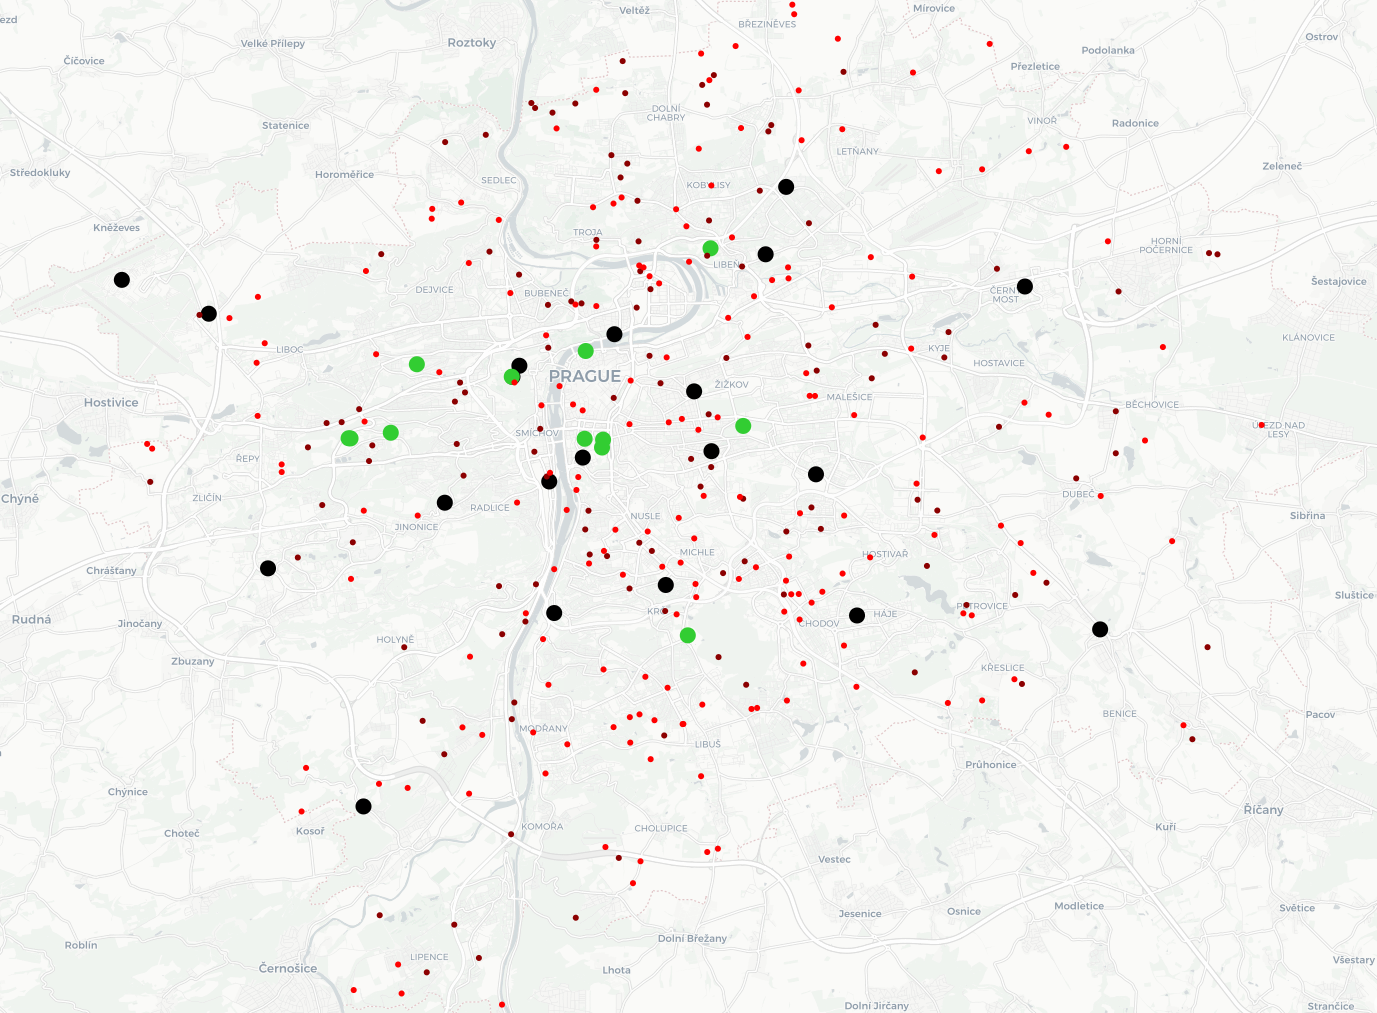
\includegraphics[width=\textwidth]{img/prague_monday_420.png}
  \centering
  \label{img:prague}
\end{figure}

Na obrázku \ref{img:prague} je znázorněno na mapě Prahy rozmístění 20 výjezdových stanic (body černé barvy), 12 nemocnic (body zelené barvy) a 300 incidentů (body červené barvy).
Tmavě červené puntíky reprezentují incidenty, které se odehrají mezi 9 a 12 hodinou.

S výše popsanou reprezentací pohotovostní služby a sady incidentů je třeba zajistit, aby simulace uměla věrohodně zjistit doby trvání příjezdů.
Připomeňme si, že simulaci používáme právě z toho důvodu, aby počet úspěšně odbavených incidentů plánem byl co nejvěrohodnější.
Věrohodnost zajistíme použitím Google API pro zjišťování těchto dob příjezdu. Konkrétně pomocí Distance Matrix API a Routes API.

V průběhu simulace je potřeba především znát následující doby příjezdů:
\begin{enumerate}
  \item z výjezdové stanice na incident,
  \item z incidentu do nemocnice,
  \item z nemocnice zpět na výjezdovou stanici.
\end{enumerate}

Simulace podporuje i tzvn. \textit{reroute}, tedy jak se záchranný tým vrací po odbavení incidentu zpět na výjezdovou stanici,
tak je povoleno, aby mohlo z aktuální lokace vyrazit na odbavování incidentu, aniž by se musela na výjezdovou stanici vrátit.

Doby příjezdů mezi výjezdovými stanicemi, incidenty a nemocnicemi si můžeme předpočítat, ale \textit{reroute} předpočítat nelze.
Můžeme si alespoň v průběhu simulování všechny spočítané doby příjezdů mezi lokacemi udržovat s přesností na desítky metrů,
aby se v budoucnu nemuselo volat Google API, což je samozřejmě pomalá operace, trvající až desítky až stovky milisekund. 

\section{Aplikace prohledávání plánů optimálními \linebreak tahy}

První metodu, kterou aplikujeme na namodelovanou záchrannou službu a incidenty podle předchozí kapitoly je algoritmus prohledávání plánů optimálními tahy \ref{alg:rekProhPlanu}.
Konkrétně použijeme jeho upravenou verzi, kde strom tahů budeme prohledávat vždy od prázdného plánu, a na každé hladině rekurze zvolíme pouze jeden náhodný optimální tah.
Oproti postupnému prohledávání všech tahů na každé úrovni má výhodu ve vyzkoušení více odlišných konfigurací a nalezené optimální plány v ceně budou s menší pravděpodobností sdílet
podobně naalokované týmy, vozidla a směny, což povede k diversifikovanějšímu prohledání množiny povolených plánů.

\begin{table}[h!]
\centering
\begin{tabular}{|c|c|c|}
\hline
\textbf{Čas běhu v minutách} & \textbf{Cena plánu} & \textbf{Odbavené incidenty} \\
\hline
7:38  & 2520055 & 295 \\
\hline
10:36 & 2325655 & 292 \\
\hline
13:23 & 2412060 & 294 \\
\hline
15:34 & 2455258 & 295 \\
\hline
17:37 & 2325654 & 288 \\
\hline
19:27 & 2505663 & 295 \\
\hline
21:20 & 2340053 & 288 \\
\hline
23:05 & 2390458 & 292 \\
\hline
24:51 & 2556061 & 295 \\
\hline
26:27 & 2325655 & 290 \\
\hline
28:10 & 2325653 & 286 \\
\hline
\end{tabular}
\caption{Spuštění prohledávání optimálními tahy na modelu Prahy.}
\label{table:optimalMovesTabulka}
\end{table}

Po spuštění metody na modelu Prahy po dobu téměř 30 minut metoda celkem navštívila 11 plánů optimálních v ceně.
Nalezený optimální plán odbavuje 295 incidentů a stojí 2455258 (viz tabulka \ref{table:optimalMovesTabulka}).

\begin{figure}[H]
  \caption{Nalezené plány metodou prohledávání plánů optimálními tahy.}
  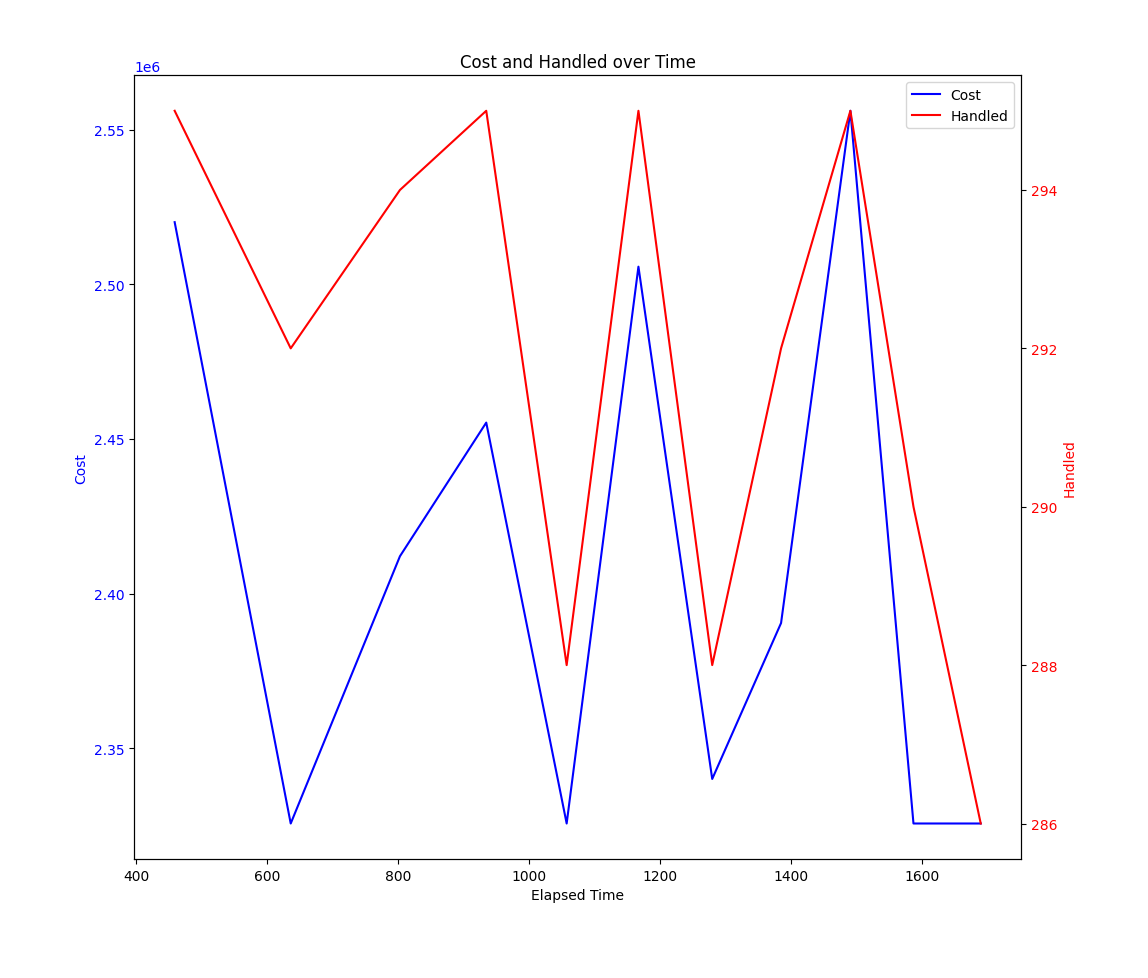
\includegraphics[width=\textwidth]{img/optimalMovesRes.png}
  \centering
  \label{img:optimalMovesRes}
\end{figure}

Na obrázku \ref{img:optimalMovesRes} vidíme vizualizovaná data z tabulky \ref{table:optimalMovesTabulka}. 
První plán trvá nalézt nejdelé, něco přes 7 minut. Důvodem je, že \textit{cache} dob příjezdů obsahuje pouze předpočítané hodnoty a musí se vykonávat větší množství
dotazů na Google API.
Při prohledávání dalších plánů už se dotazuje na Google API mnohem méně často.

Metoda navštívila pro každý plán optimální v ceně při jeho budování jeden plán pro každý incident, čili celkové navštívila $11 \cdot 300 = 3300$ plánů.
Celkový počet dotazů na dobu trvání příjezdu je 133189050, kde pro 133179688 případu, tedy $99.99\%$, byla doba příjezdu předpočítaná a vrácena z \textit{cache}.

\section{Aplikace lokálního prohledávání}

V této kapitole aplikujeme na model Prahy lokální prohledávání (viz kapitola \ref{kap:localSearch}).
Použijeme ho přesně jak je popsaný algoritmem \ref{alg:hillclimb}.
Prohledávání začneme z prázdného plánu a jako účelovou funkci použijeme váženou sumu ceny plánu a počtu odbavených incidentů (viz definice \ref{df:vazenaSumaUcelF}), s $\alpha = 0.99$, abychom
upřednostňovali plány s vyšším počtem odbavených incidentů.

\begin{figure}[H]
  \caption{Nalezené plány metodou lokálního prohledávání plánů.}
  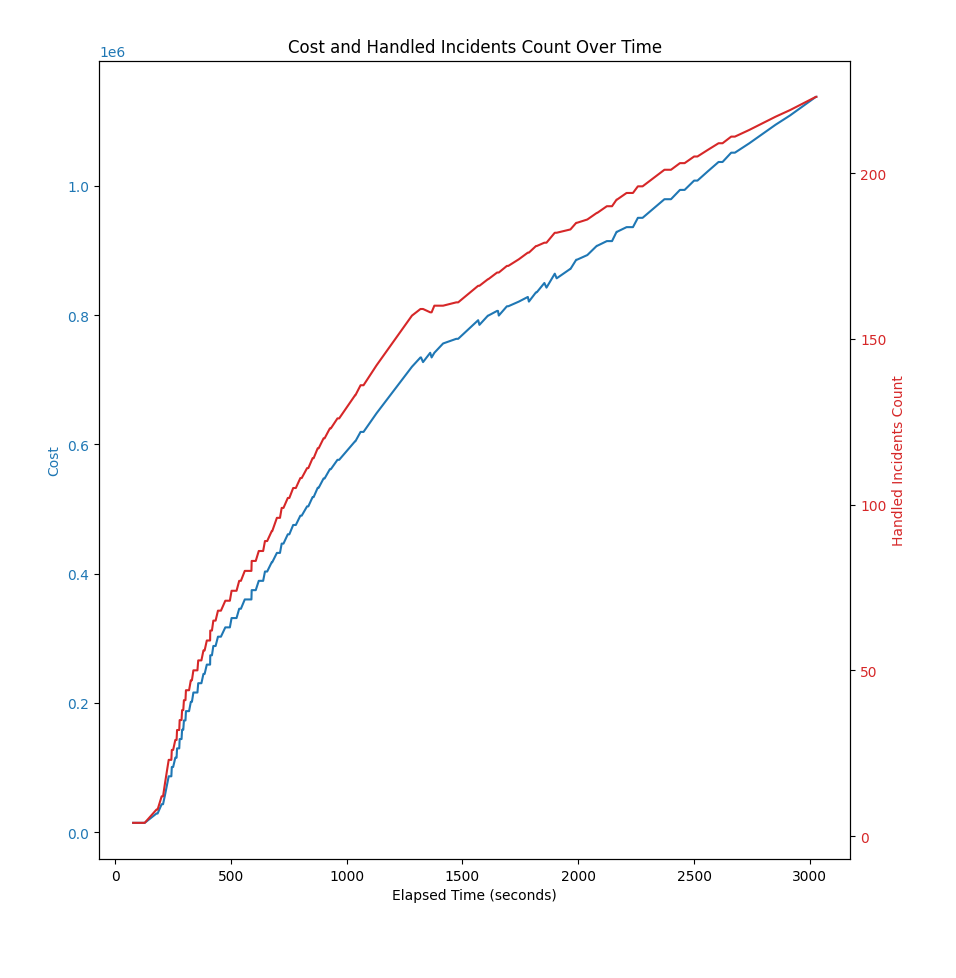
\includegraphics[width=\textwidth]{img/local_search_empty_plan_plot.png}
  \centering
  \label{img:localSearchRes}
\end{figure}

Na obrázku \ref{img:localSearchRes} vidíme jak se aktuální plán mění v čase.
Lokální prohledávání bylo spuštěné po dobu 50 minut, a pak bylo přeřušeno. 
Nejlepší nalezený plán po 50 minutách úspěšně odbaví 223 incidentů z 300 incidentů a stojí 137673.
To je v porovnání s předchozí metodou, která za pouhých 7 minut nalezla plán odbavující 295 incidentů nedostačující výsledek.
I když by se podle růstu křivky dalo usoudit, že by metoda lokálního prohledávání také byla schopná nalézt dost dobrý plán, trvalo by to příliš dlouho.

Lokální prohledávání celkem navštívilo 22997 plánů. To je až 7 krát tolik, kolik plánů navštívila metoda prohledávání optimálními tahy.
Lokální prohledávání tedy není vhodné na budování optimálního plánu z prázdného plánu, protože zbytečně navštíví velké množství plánů a trvá tak zbytečně dlouho.

Můžeme si polepšit, sice že začneme prohledávát ne z prázdného plánu, ale z plánu zvoleného nějak chytře. Z plánu, který už je skoro optimální a lokální Prohledávání
už jej jenom doladí.

Jednou z možností jak takový startovní plán zvolit je použít první nalezený optimální plán v ceně předchozí metodou a na něj spustit lokální prohledávání.

\begin{figure}[H]
  \caption{Nalezené plány metodou lokálního prohledávání plánů z plánu optimálního v ceně.}
  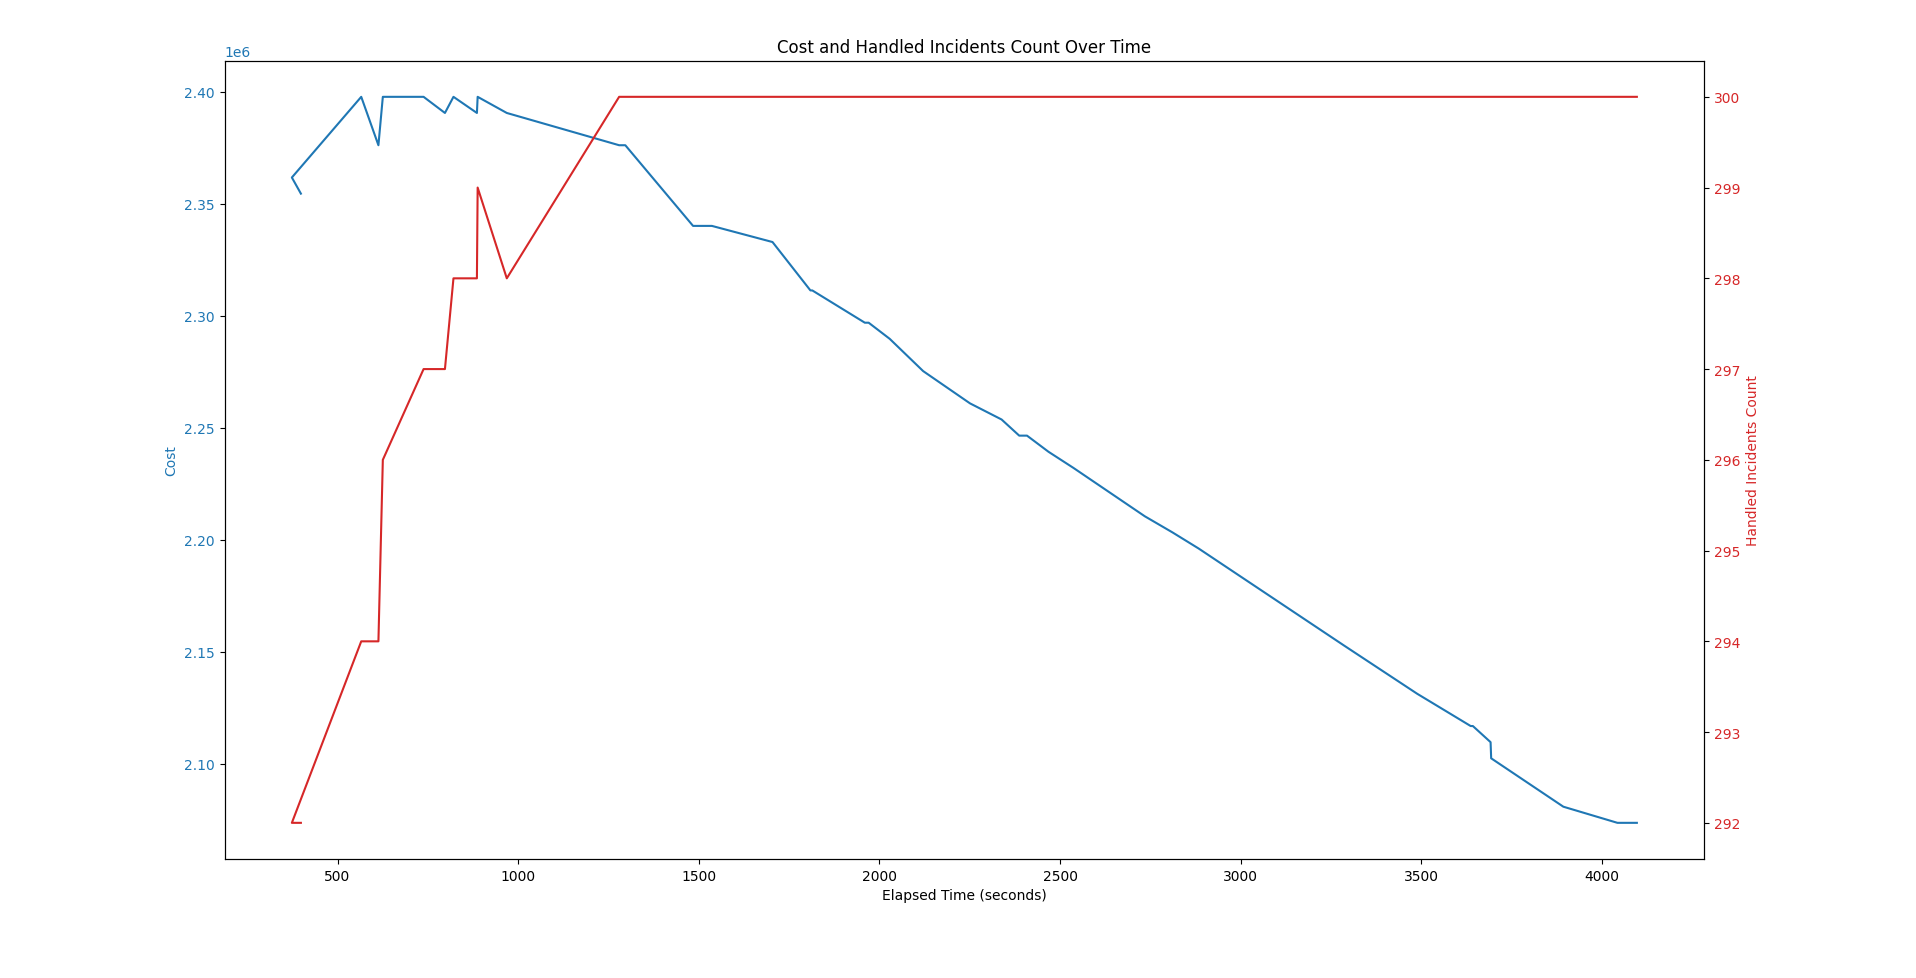
\includegraphics[width=\textwidth]{img/hybrid_prague.png}
  \centering
  \label{img:hybrid}
\end{figure}

Na obrázku \ref{img:hybrid} vidíme graf, kde lokální prohledávání začíná ne z prázdného plánu, ale z plánu optimálního v ceně.
Můžeme vidět, že lokální prohledávání upravuje plán tak, že postupně odbavuje více incidentů, až nakonec všech 300. Poté už jen postupně snižuje cenu plánu.
Po 20 minutách nalezne plán odbavující všechny incidenty a zhruba po hodině lokální prohledávání stagnuje a nalezne lokální optimum.


\section{Aplikace tabu prohledávání}

V této kapitole aplikujeme na model Prahy tabu prohledávání (viz kapitola \ref{kap:tabuSearch}).
Tabu prohledávání je v podstatě lokální prohledávání s pamětí, podle které umí sofistikovaněji vybrat sousední plán,
pokud se ocitne v lokálním optimu.
Z toho důvodu bude podobně jako u lokálního prohledávání trvat příliš dlouho, než nalezne nějaký dost dobrý plán, pokud bychom tabu prohledávání pustili z prázdného plánu.
Nemá proto smysl pouštět tabu prohledávání z prázdného plánu a pustíme tabu prohledávání rovnou z nějakého už dost dobrého plánu.
Tím bude stejně jako u lokálního prohledávání plán optimální v ceně.

\begin{figure}[H]
  \caption{Nalezené plány tabu metodou z plánu optimálního v ceně.}
  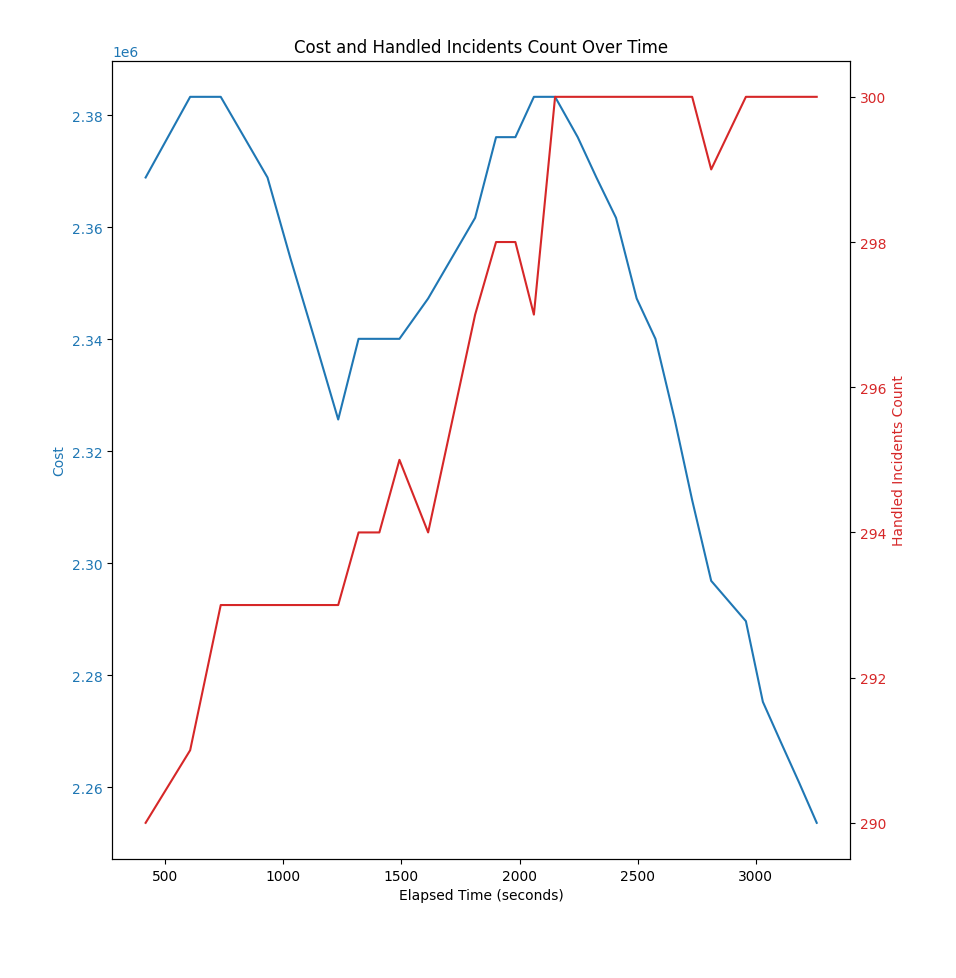
\includegraphics[width=\textwidth]{img/prague_hybrid_tabu.png}
  \centering
  \label{img:hybrid_tabu}
\end{figure}

Na obrázku \ref{img:hybrid_tabu} vidíme doposud nejlepší plány nalezené tabu metodou v čase.
Nalézt plán odbavující všech 300 incidentů trvá kolem 30 minut, což je o 10 minut déle, než trvalo lokálnímu prohledávání. 
To je pochopitelné, protože při navštívení každého souseda, kterých bude obdobně jako u lokálního prohledávání, se musí kontrolovat,
zda není obsažen v tabu. Proto vyhodnocení souseda bude trvat o něco déle, což se při tak velkém množství navštívených plánů poměrně rychle nasčítá.

Tabu prohledávání bylo puštěno něco kolem hodiny, a obdobně jako u lokálního prohledávání, s roustoucí délkou běhu programu se i snižuje cena plánu.
Výhoda tabu prohledávání je hlavně v schopnosti nezůstat v lokálním optimu a umět robustněji prohledávat prostor konfigurací.
Tato výhoda v našem případě ale není využita, protože tabu prohledávání ani za hodinu běhu na lokální optimum nenarazilo.
Spíše naopak, prohledávání tabu je nevýhodou, a lokální prohledávání jako rychlejší metodu je v tomto případě lepší volbou.


\section{Aplikace simulovaného žíhání}

\section{Porovnání metod}

